%!TEX program = xelatex

\documentclass{article}
% \usepackage[utf8]{inputenc}
\usepackage[UTF8]{ctex}
\usepackage{indentfirst}
\usepackage{lmodern}% http://ctan.org/pkg/lm
\usepackage{setspace}
\usepackage{verbatim}
\usepackage{amsmath}%数学
\usepackage{amsthm}%数学定理、证明
\usepackage{graphicx}%graphicx基于graphics,更方便
% \usepackage{subfig}%图像
\usepackage{subfigure}
\usepackage{booktabs}%表格
\usepackage{tabularx}%表格
\usepackage{multirow}
\usepackage{multicol}
\usepackage{listings}
\usepackage{relsize}
\usepackage[usenames]{color}   
\usepackage{fontspec}

%\usepackage{colortbl}%表格颜色
\usepackage[table]{xcolor}
\usepackage{array}
\usepackage[rightcaption]{sidecap}
\usepackage{hyperref}
\usepackage{float}
\hypersetup{
colorlinks=true,
linkcolor=black
}%解决目录红框问题
\lstset{
         language = vhdl, numbers=left, 
         numberstyle=\tiny,keywordstyle=\color{blue!70},
         commentstyle=\color{red!50!green!50!blue!50},frame=shadowbox,
         rulesepcolor=\color{red!20!green!20!blue!20},basicstyle=\ttfamily
}
\newcommand{\myd}{\;\mathrm{d}}%自定义积分变量命令
% \renewcommand{\listtablename}{表格}%改变listoftable的名字
\renewcommand{\arraystretch}{1.8}%The height of each row, relative to its default height
% \setmonofont{Consolas}
\renewcommand\refname{参考网站}
% \setlength{\tabcolsep}{18pt}%The space between the text and the left/right border of its containing cell
% \setlength{\arrayrulewidth}{0.4mm}%sets the thickness of the borders of the table


\setlength{\parindent}{2em}%控制首行缩进
\addtolength{\parskip}{3pt}%\parskip 控制段落(paragraph)距离
%\singlespacing%单倍行距
%\doublespacing%双倍行距
%\setstretch{1.25}%设置行距为1.25
\onehalfspacing %1.5倍行距
%\begin{doublespacing} 行距环境 \end{doublespacing}
\graphicspath{{./figures/}} % 指定图片所在文件夹
%\newtheorem{definition}[定义]{section}
%定制环境: {环境名}[编号延续]{显示名}[编号层次]

\begin{document}
\begin{titlepage}
        \vspace*{-3cm}
	
	\begin{figure}[h]
		\centering
		
\includegraphics[width=0.7\linewidth]{zjdx}
	\end{figure}

	\vspace*{0.5cm}
	\begin{figure}[h]
		\centering
		
\includegraphics[width=0.5\linewidth]{QSY}
	\end{figure}
	\vspace{-0.5cm}
	\begin{center}
		\Huge{\textbf{数字电路分析与设计}}\\
		
		\Huge{\textbf{实验报告}}
	\end{center}
	
	\vspace*{0.5cm}


	\vspace*{1cm}
    \begin{center}
            \Large 实验名称\ \ \underline{\makebox[250pt]{四位二进制加法器设计}} \\ 
            \vspace{0.3cm}
            \Large 姓名 \ \ \underline{\makebox[220pt]{小黄}} \\ 
            \vspace{0.3cm}
            学  号\ \ \underline{\makebox[220pt]{3100100000}}\\
            \vspace{0.3cm}
            实验地点\ \ \underline{\makebox[250pt]{浙江大学紫金港校区}}\\
            \vspace{0.3cm}
            实验日期\ \ \underline{\makebox[250pt]{2020年 5 月 25 日}}\\
            % \vspace{0.3cm}
            % 指导老师\ \ \underline{\makebox[250pt]{郑晓东、徐建锋、蒋凌颖、吕玮阁}}\\
            

             
    \end{center}
        
    
\end{titlepage}

\newpage
% \setcounter{tocdepth}{5}
\tableofcontents
\thispagestyle{empty}%Removes the page numbering.
\listoffigures%生成插图
% \listoftables%生成表格
\thispagestyle{empty}%Removes the page numbering.

\newpage
\pagenumbering{arabic}%重新开始标号,阿拉伯数字形式


\section{实验目的}
\begin{itemize}
 \item 熟悉 Quartus II 软件的使用
 \item 掌握逻辑功能的 VHDL 语言描述和原理图描述的方法
 \item 进一步掌握四位串行二进制加法器的设计方法
 \item 掌握用仿真波形验证电路功能的方法

\end{itemize}

\section{实验内容}
\begin{itemize}
\item 利用原理图实现简易与非门电路
\item 利用VHDL实现与非门电路
\item 利用原理图和VHDL实现奇偶位判断电路
\item 用原理图方式描述4位全加器的功能
\item 通过波形仿真验证4位全加器的功能
\end{itemize}




\section{实验原理}
\subsection{奇偶位判断电路}
判断1的个数,奇数个1输出1,偶数个1输出0。对于4位二进制奇偶位判断电路,利用卡诺图可以得到,若输入为 $ABCD$, 则输出应为$A\oplus B\oplus C\oplus D$,可以用两个这样的电路拓展到八位奇偶位判断。
利用原理图的方式用两个4位异或电路实现8位异或,然后底层的4位异或利用VHDL实现。

\subsection{全加器}
通过列出卡诺图我们可以得到全加器的输入和输出:
$$
\begin{aligned}
 S&=A\oplus B \oplus C_{i-1}\\
 C_i&={AB+BC_{i-1}+AC_{i-1}}
\end{aligned}
$$
\subsection{4位串行进位二进制全加器}
4位串行进位二进制全加器以1位全加器的设计为基础,
将四个1位二进制全加器串接即可构成四位二进制全加器;


在使用Quartus构建时,顶层采用原理图描述,底层采用VHDL语言描述,


串行连接所依据的式子如下(由于实验中标号从1开始的,这里的原理也按下标从1开始)
\begin{center}
\begin{tabular}{lr}
&$A_4A_3A_2A_1$\\
+&$B_4B_3B_2B_1$\\
\text{进位}&\tiny $C_3$\; \tiny $C_2$\; \tiny $C_1$\quad\\
\hline
&$C_4S_4S_3S_2S_1$
\end{tabular}
\end{center}


实验原理图如下:
\begin{figure}[H]
\centering
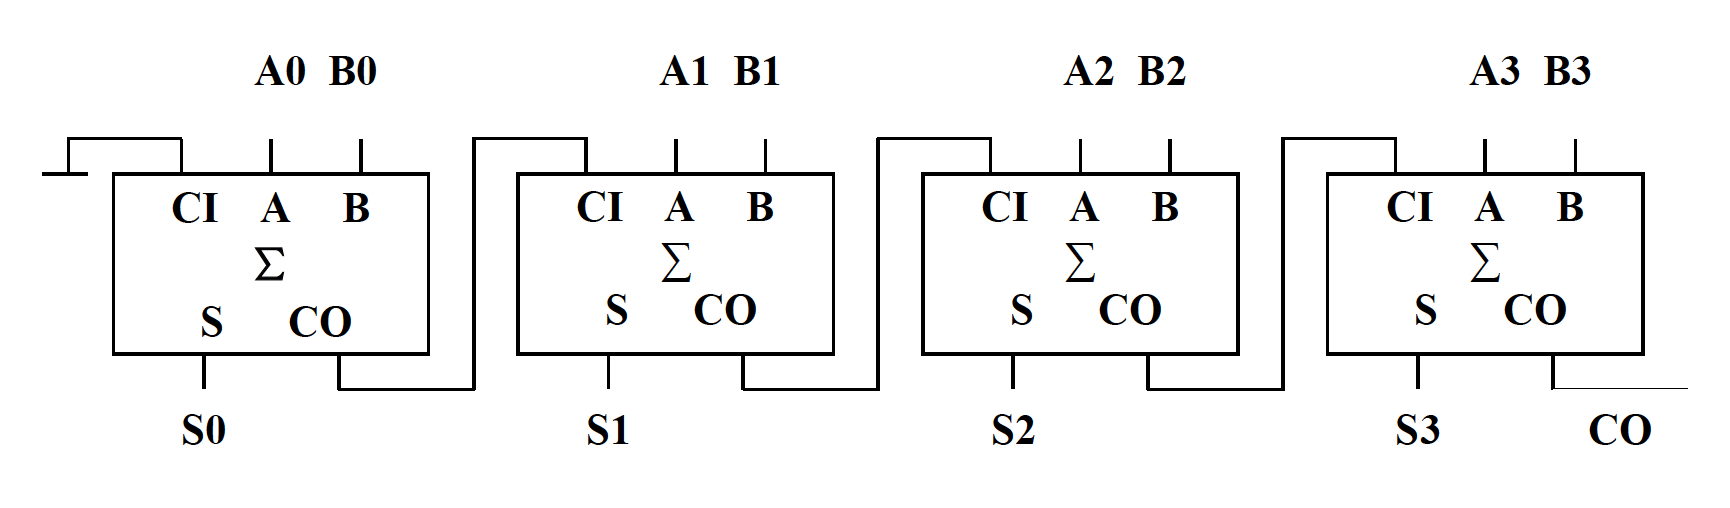
\includegraphics[width=\textwidth]{p1.png}
\caption{实验原理图}
\end{figure}


\section{简单的二位与非门实现}
本实验的目的是熟悉Quartus软件。
\subsection{用原理图实现}
\begin{figure}[H]
\centering
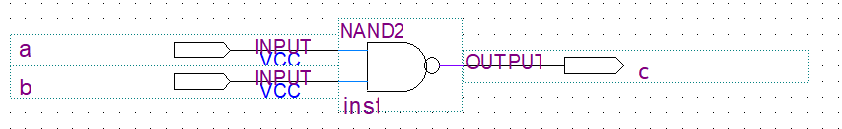
\includegraphics[width=\textwidth]{nand2_layout}
\caption{原理图实现nand2}
\end{figure}
\begin{figure}[H]
\centering
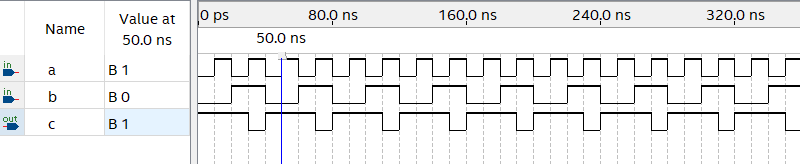
\includegraphics[width=\textwidth]{nand2_output1}
\caption{nand2仿真结果1}
\end{figure}
\subsection{用VHDL实现}
\begin{lstlisting}
-- nand2 
library ieee;
use ieee.std_logic_1164.all;
entity nand2_3 is
port(a,b:in std_logic; z:out std_logic);
end nand2_3;
architecture a1 of nand2_3 is
begin 
  z<=not(a and b);
  end a1;
\end{lstlisting}
\begin{figure}[H]
\centering
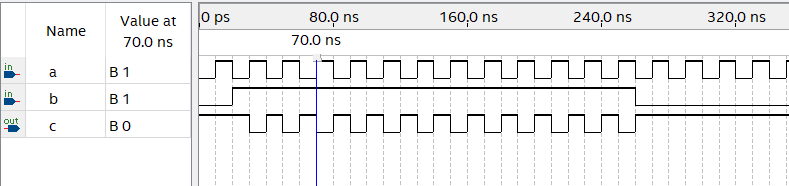
\includegraphics[width=\textwidth]{nand2_output2}
\caption{nand2仿真结果2}
\end{figure}
可见,我们实现了预期与非的功能(只有11输出0)。
\section{奇偶位判断实验}
\subsection{原理图实现}
\begin{figure}[H]
\centering
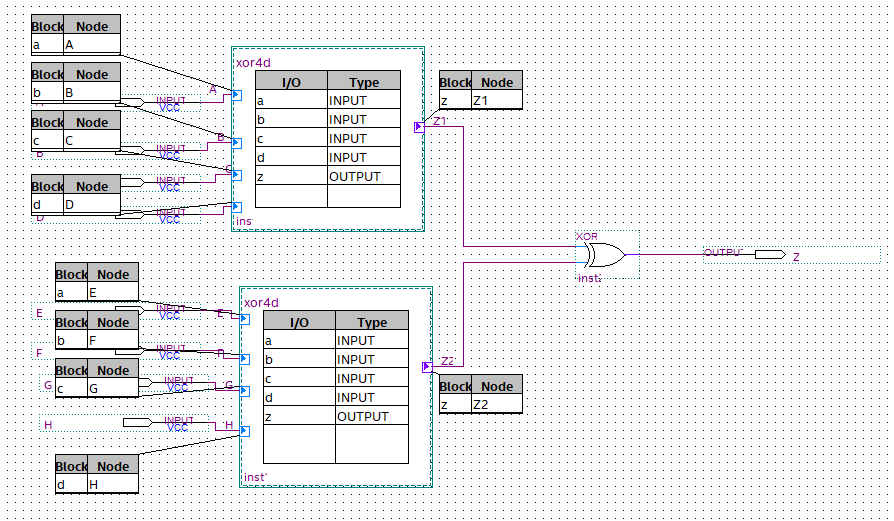
\includegraphics[width=\textwidth]{xor8d_layout}
\caption{xor8d原理图实现}
\end{figure}
\subsection{底层xor4d的代码}
\begin{lstlisting}
-- xor4d
LIBRARY ieee;
USE ieee.std_logic_1164.all;


--  Entity Declaration

ENTITY xor4d IS
-- {{ALTERA_IO_BEGIN}} DO NOT REMOVE THIS LINE!
PORT
(
a : IN STD_LOGIC;
b : IN STD_LOGIC;
c : IN STD_LOGIC;
d : IN STD_LOGIC;
z : OUT STD_LOGIC
);
-- {{ALTERA_IO_END}} DO NOT REMOVE THIS LINE!

END xor4d;


--  Architecture Body

ARCHITECTURE xor4d_architecture OF xor4d IS


BEGIN
z<= a xor b xor c xor d;

END xor4d_architecture;
\end{lstlisting}
\subsection{仿真结果}
\begin{figure}[H]
\centering
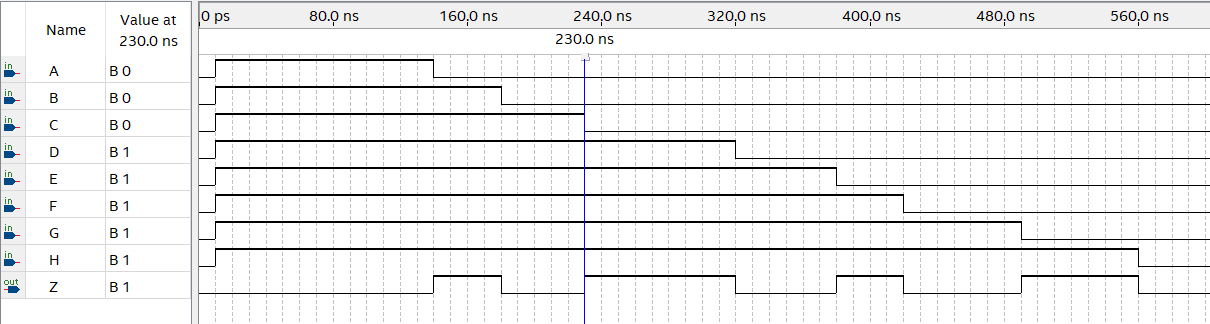
\includegraphics[width=\textwidth]{xor8d_output}
\caption{xor8d仿真结果}
\end{figure}
可见,我们实现了预期奇偶位判断的功能:奇数个1输出1,否则输出0。
\section{4位全加器实验}

\subsection{创建4位串行二进制全加器原理图}
在Quartus中的连接图如下:
\begin{figure}[H]
\centering
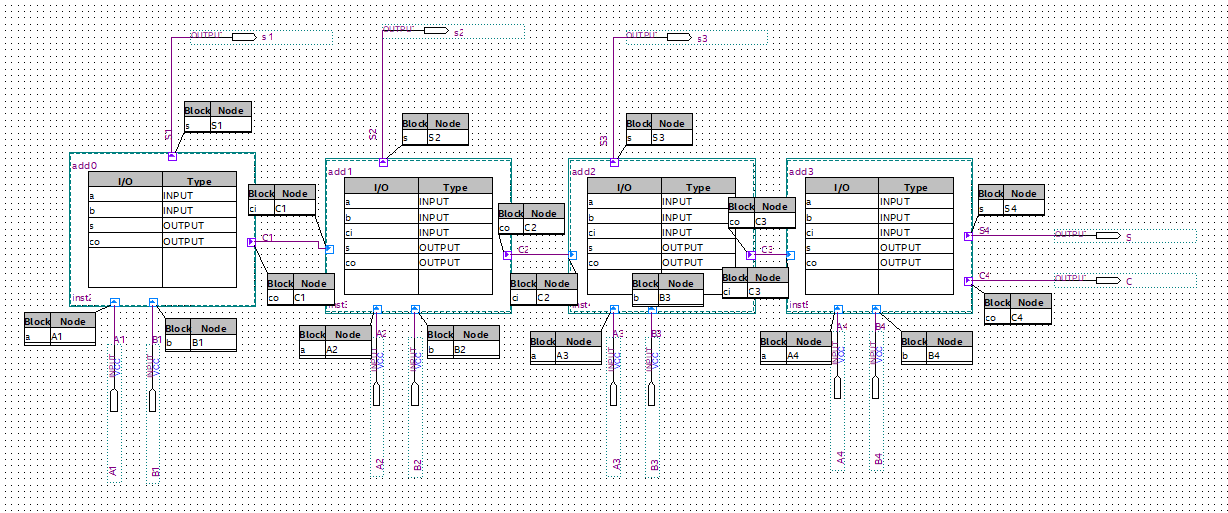
\includegraphics[width=\textwidth]{layout}
\caption{adder4原理图实现}
\end{figure}
\subsection{创建1位二进制全加器的VHDL源文件}
实验代码如下。
\begin{lstlisting}
-- add0

LIBRARY ieee;
USE ieee.std_logic_1164.all;

--  Entity Declaration

ENTITY add0 IS
-- {{ALTERA_IO_BEGIN}} DO NOT REMOVE THIS LINE!
PORT
(
a : IN STD_LOGIC;
b : IN STD_LOGIC;
s : OUT STD_LOGIC;
co : OUT STD_LOGIC
);
-- {{ALTERA_IO_END}} DO NOT REMOVE THIS LINE!

END add0;


--  Architecture Body

ARCHITECTURE add0_architecture OF add0 IS


BEGIN
s<=a xor b;
co <= a and b;
END add0_architecture;


-- add1 add2 add3
LIBRARY ieee;
USE ieee.std_logic_1164.all;


--  Entity Declaration

ENTITY add1 IS
-- {{ALTERA_IO_BEGIN}} DO NOT REMOVE THIS LINE!
PORT
(
a : IN STD_LOGIC;
b : IN STD_LOGIC;
ci : IN STD_LOGIC;
s : OUT STD_LOGIC;
co : OUT STD_LOGIC
);
-- {{ALTERA_IO_END}} DO NOT REMOVE THIS LINE!

END add1;


--  Architecture Body

ARCHITECTURE add1_architecture OF add1 IS


BEGIN
s <= a xor b xor ci;
co <= (a and b) or (b and ci) or (a and ci);
END add1_architecture;


\end{lstlisting}

\subsection{4位二进制全加器仿真测试}

\begin{enumerate}
\item 新建一个仿真波形文件
\item 添加需要仿真的输入、输出信号
\item 给输入信号设置仿真激励
\item 点击工具栏中的图标启动波形仿真过程
\item 观察仿真结果
\end{enumerate}

仿真结果如下:
\begin{figure}[H]
\centering
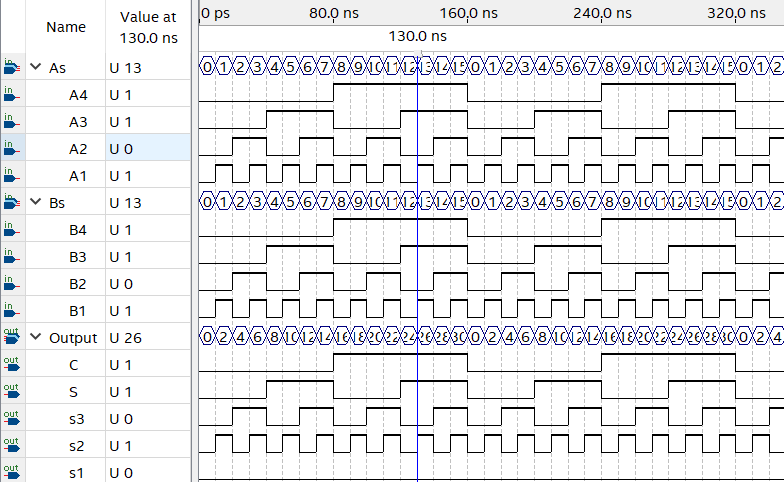
\includegraphics[width=\textwidth]{sum_output}
\caption{adder4仿真结果}
\end{figure}
可见,我们实现了4位二进制加法!
% \newpage
% 参考网站
% \begin{thebibliography}{9}%参考文献条目编号的宽度
% \bibitem{b1}
%   https://www.dxomark.com/cn/
% \bibitem{b2}
%   https://www.apple.com.cn/
% \end{thebibliography}


\end{document}

%好看的颜色 [HTML] 淡蓝色 CBF5FB
%>{\columncolor[HTML]{AAACED}} 列背景颜色
%\rowcolor, \cellcolor 行背景、单元背景颜色
